%%%%%%%%%%%%%%%
% This file is concerned with the system sequence diagram,
% a subsection of the functional requirements.
%
% Please remember to compile the document from "00_finalreport.tex".
% It will not work otherwise.
%%%%%%%%%%%%%%%

	\subsection{System Sequence Diagram}
	
		\subsubsection{Diagram}
			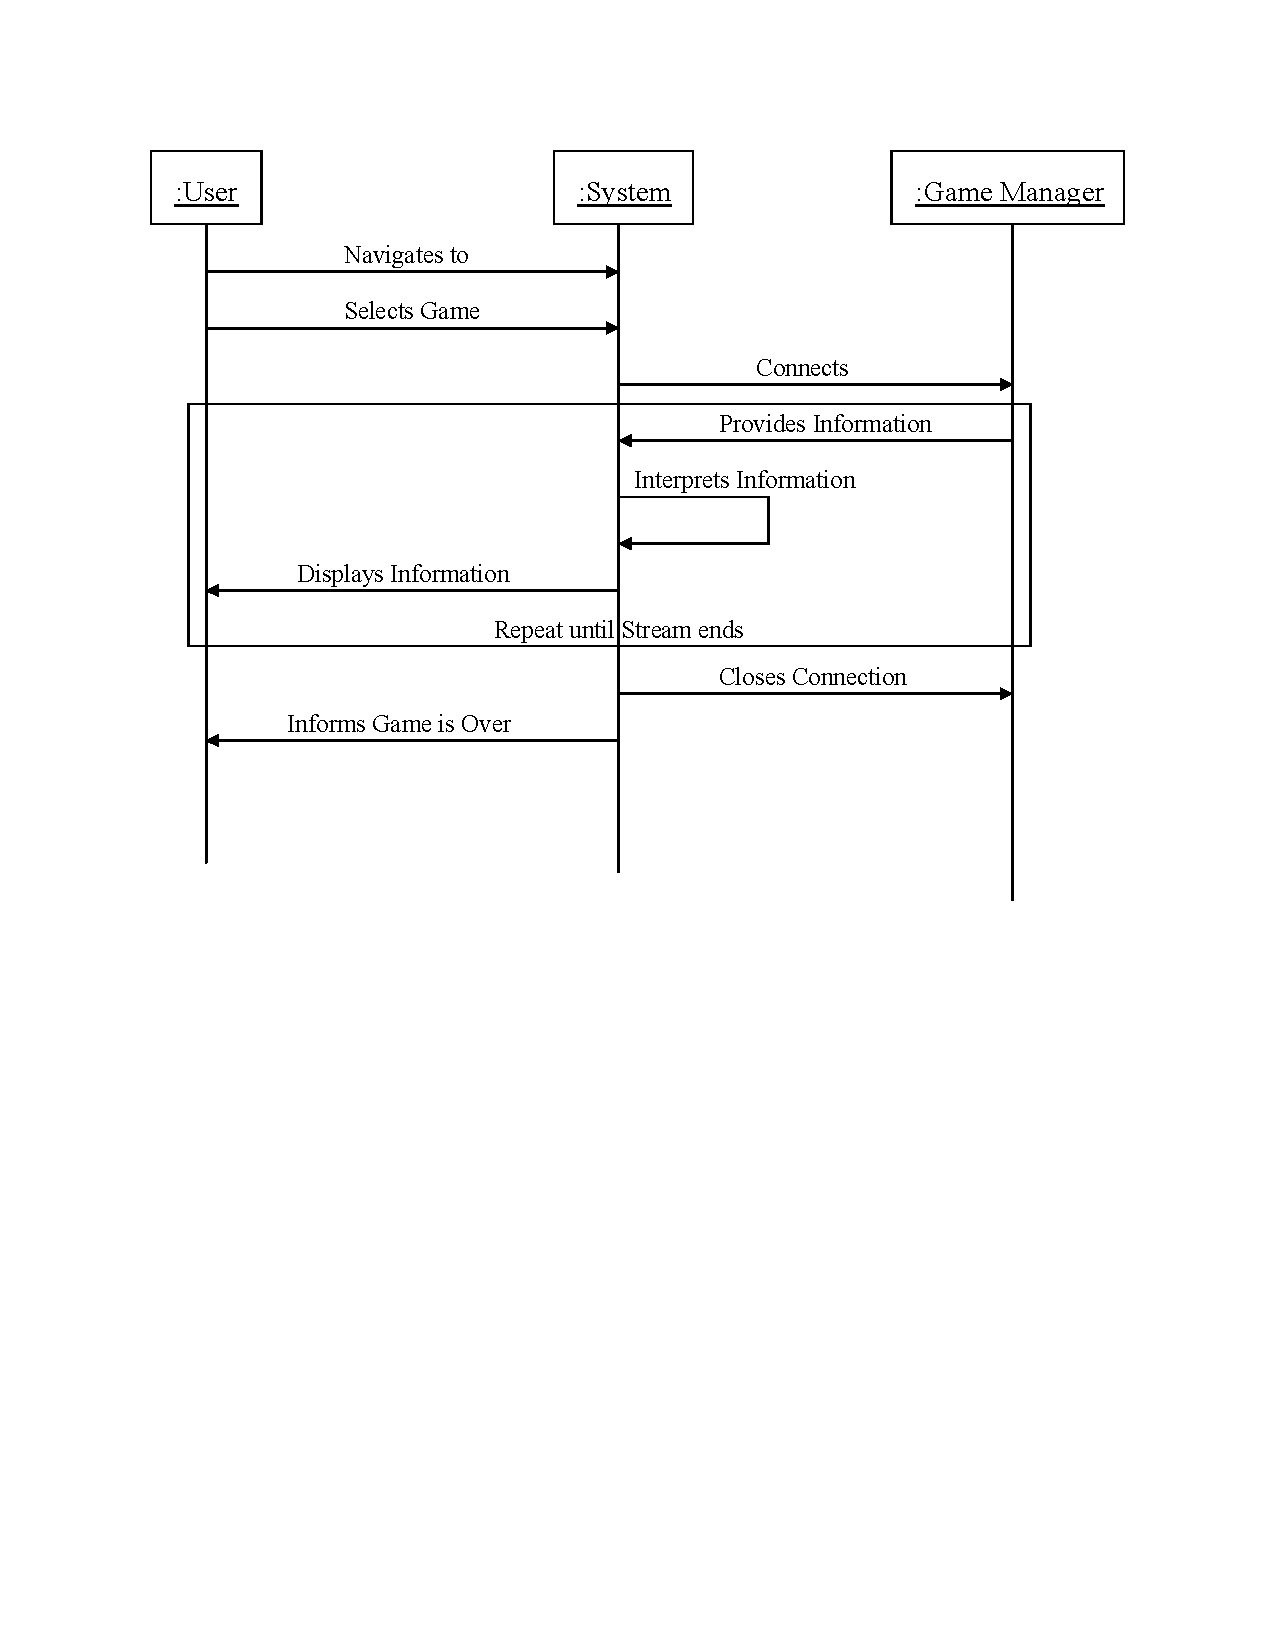
\includegraphics[width=1.0\textwidth]{./SSD_of_Watch_Live.pdf}
			
		\subsubsection{Description}
			The diagram starts with the Person, a normal human being. The person interacts with the system (in the sense that the person is clicking links on the website and typing in fields). The System is in control of the general running of the domain. When a person wants to register or sign-in to the site, they are interacting with the Form, not directly to the database. The form is in control of handing the entered info(either login info or registration info) to the database. The User DB contains Users, being a class of Person. When the user requests to see a game, The Game Manager is pinged to pull up specific information, either Past Games or Live Games, recieving information from a Games database. the actual game data is presented from the databases maintained by the server group and outside the scope of this paradigm.
